% !TEX program = xelatex
\documentclass[a4paper,14pt,oneside,openany]{memoir}

\usepackage[left=30mm, right=15mm, top=20mm, bottom=20mm]{geometry}
\pagestyle{plain}
\parindent=1.25cm
\usepackage{indentfirst}

\usepackage{polyglossia}
\setdefaultlanguage[indentfirst=true,forceheadingpunctuation=false]{russian}
\setotherlanguages{english}

\IfFontExistsTF{Times New Roman}
{\setmainfont{Times New Roman}
\newfontfamily\cyrillicfont{Times New Roman}[Script=Cyrillic]}
{\setmainfont[Script=Cyrillic]{FreeSerif}}

\IfFontExistsTF{Courier New}
{\setmonofont{Courier New}
\newfontfamily\cyrillicfonttt{Courier New}[Script=Cyrillic]}
{\setmonofont[Script=Cyrillic]{FreeMono}}

\IfFontExistsTF{Arial}
{\setsansfont{Arial}
\newfontfamily\cyrillicfontsf{Arial}[Script=Cyrillic]}
{\setsansfont[Script=Cyrillic]{FreeSans}}

\setsecnumdepth{subsection}
\renewcommand*{\chapterheadstart}{}
\renewcommand*{\printchaptername}{}
\renewcommand*{\chapnumfont}{\normalfont\bfseries}
\renewcommand*{\afterchapternum}{\hspace{1em}}
\renewcommand*{\printchaptertitle}{\normalfont\bfseries\centering\MakeUppercase}
\setbeforesecskip{20pt} \setaftersecskip{20pt}
\setsecheadstyle{\raggedright\normalfont\bfseries}
\setbeforesubsecskip{20pt} \setaftersubsecskip{20pt}
\setsubsecheadstyle{\raggedright\normalfont\bfseries}

\addto\captionsrussian{\renewcommand\contentsname{Содержание}}
\setrmarg{2.55em plus1fil}
\renewcommand{\aftertoctitle}{\afterchaptertitle \vspace{-\cftbeforechapterskip}}
\renewcommand*{\cftchapternumwidth}{1.5em}
\renewcommand*{\cftchapterfont}{\normalfont\MakeUppercase}
\renewcommand*{\cftchapterpagefont}{\normalfont}
\renewcommand*{\cftchapterdotsep}{\cftdotsep}
\renewcommand*{\cftdotsep}{1}
\renewcommand*{\cftchapterleader}{\cftdotfill{\cftchapterdotsep}}
\maxtocdepth{subsection}

\tolerance 1414
\hbadness 1414
\emergencystretch 1.5em
\hfuzz 0.3pt
\vfuzz \hfuzz
\clubpenalty=10000
\widowpenalty=10000
\brokenpenalty=4991

\makeatletter
    \def\russian@Alph#1{\ifcase#1\or
       А\or Б\or В\or Г\or Д\or Е\or Ж\or
       И\or К\or Л\or М\or Н\or
       П\or Р\or С\or Т\or У\or Ф\or Х\or
       Ц\or Ш\or Щ\or Э\or Ю\or Я\else\xpg@ill@value{#1}{russian@Alph}\fi}
    \def\russian@alph#1{\ifcase#1\or
       а\or б\or в\or г\or д\or е\or ж\or
       и\or к\or л\or м\or н\or
       п\or р\or с\or т\or у\or ф\or х\or
       ц\or ш\or щ\or э\or ю\or я\else\xpg@ill@value{#1}{russian@alph}\fi}
\makeatother

\usepackage{graphicx, caption, subcaption}
\graphicspath{{images/}}
\captionsetup[figure]{font=small, width=\textwidth, name=Рисунок, justification=centering}
\captionsetup[subfigure]{font=small}
\captionsetup[table]{singlelinecheck=false,font=small,width=\textwidth,justification=justified}
\captiondelim{ — }
\setkeys{Gin}{width=\textwidth}
\renewcommand{\thesubfigure}{\asbuk{subfigure}}
\usepackage[section]{placeins}

\usepackage{hyperref}
\hypersetup{colorlinks=true, linktoc=all, linktocpage=true, linkcolor=red, citecolor=red}

\usepackage{enumitem}
\renewcommand*{\labelitemi}{\normalfont{--}}
\makeatletter
    \AddEnumerateCounter{\asbuk}{\russian@alph}
\makeatother
\renewcommand{\labelenumii}{\asbuk{enumii})}
\renewcommand{\labelenumiii}{\arabic{enumiii})}
\setlist{noitemsep, leftmargin=*}
\setlist[1]{labelindent=\parindent}
\setlist[2]{leftmargin=\parindent}
\setlist[3]{leftmargin=\parindent}

\counterwithout{figure}{chapter}
\counterwithout{equation}{chapter}
\counterwithout{table}{chapter}

\usepackage{xcolor}
\usepackage{listings}
\usepackage{float}
\usepackage{longtable,ltcaption}
\usepackage{multirow,makecell}
\usepackage{booktabs}
\usepackage{soulutf8}
\usepackage{icomma}
\usepackage{hyphenat}
\usepackage{textcomp}
\usepackage{amsmath}

% Уменьшаем кегль листингов, чтобы длинные строки кода влезали в поле набора
\makeatletter
\def\verbatim@font{\normalfont\ttfamily\footnotesize}
\makeatother

\begin{document}

% ------------------------- Титульный лист -------------------------
\thispagestyle{empty}
\begin{center}
    МИНИСТЕРСТВО ЦИФРОВОГО РАЗВИТИЯ, СВЯЗИ И МАССОВЫХ КОММУНИКАЦИЙ \\ РОССИЙСКОЙ ФЕДЕРАЦИИ
    \vspace{20pt}
    Федеральное государственное бюджетное образовательное учреждение \\ высшего образования \\
    "Сибирский государственный университет телекоммуникаций и информатики" \\
    \vspace{20pt}
    Кафедра телекоммуникационных систем и вычислительных средств (ТС и ВС)
\end{center}
\vfill
\begin{center}
    ЛАБОРАТОРНАЯ РАБОТА №7 \\
    по дисциплине \\
    \textit{"Теория массового обслуживания"}
    \vspace{20pt}
    по теме: \\
    \uppercase{СМО G/G/1. Исследование зависимостей параметров \\ от типа функций распределения управляющих последовательностей}
\end{center}
\vfill
\noindent Студент: группа № ИКС-431 \hfill В.П. Салий

\vspace{20pt}

\noindent Преподаватель: \hfill А.В. Андреев
\vfill
\begin{center}
    Новосибирск 2026 г.
\end{center}

\newpage
\setcounter{page}{2}
\OnehalfSpacing*

% ------------------------- Цель -------------------------
\chapter*{Цель работы}
\addcontentsline{toc}{chapter}{Цель работы}
Моделирование поведения системы массового обслуживания и сравнение аналитических и статистических оценок стационарных характеристик для различных видов управляющих последовательностей (законов распределения входного потока и времени обслуживания).

% ------------------------- Основная глава -------------------------
\chapter{СМО G/G/1. Влияние типа распределения управляющих последовательностей}
\label{ch:lab7}

\section*{Задание}
\addcontentsline{toc}{section}{Задание}
Используя управляющие последовательности, сформированные в лабораторной работе №6 ($\tau$, $\tau_1$ --- интервалы между заявками; $\nu$, $\nu_1$ --- времена обслуживания), получить и исследовать четыре модели одноканальных СМО с неограниченной очередью и дисциплиной FIFO:
\begin{itemize}
    \item M/M/1 --- $(\tau, \nu)$: показательный вход и показательное обслуживание;
    \item M/G/1 --- $(\tau, \nu_1)$: показательный вход, произвольное (гамма) обслуживание;
    \item G/M/1 --- $(\tau_1, \nu)$: произвольный (гамма) вход, показательное обслуживание;
    \item G/G/1 --- $(\tau_1, \nu_1)$: произвольные вход и обслуживание.
\end{itemize}
Значения $\lambda$ и $\mu$ выбрать из условия стационарности. Для каждой модели получить зависимости: числа пришедших и обслуженных заявок от времени; числа заявок в СМО от времени; распределения числа заявок в СМО. Рассчитать характеристики: коэффициент загрузки $\rho$, среднее число заявок $N$, среднее время ожидания $W$, среднее время пребывания $T$. Сравнить результаты, сделать выводы. Вариант 18.

\section{Теоретические сведения}

\subsection{Обозначения СМО и управляющие последовательности}

В обозначении Кендалла $A/B/1$ первая буква задаёт закон распределения интервалов входного потока, вторая --- закона обслуживания; $M$ --- показательное (экспоненциальное) распределение, $D$ --- детерминированное, $G$ --- произвольное. Модель приводится в действие дискретно-событийной имитацией: для каждой заявки фиксируются моменты поступления $t_i=\sum_{k\le i}\tau_k$ и окончания обслуживания, при этом поддерживается один прибор и FIFO-очередь.

\subsection{Характеристики и условие стационарности}

Коэффициент загрузки $\rho=\lambda/\mu<1$ --- условие стационарности. По формуле Литтла среднее число заявок в системе $N=\lambda T$, в очереди $N_q=\lambda W$, где $T$ --- среднее время пребывания, $W$ --- среднее время ожидания. Показательное распределение имеет наибольшую дисперсию ($C^2=1$) среди рассматриваемых, поэтому системы с $M$-компонентами дают бо\'льшие очереди; более «регулярные» (гамма с меньшей дисперсией) вход и обслуживание уменьшают среднее число заявок.

\section{Выполнение работы}

Параметры взяты из лабораторной работы №6: $\lambda=0{,}8$, $\mu=1{,}0$ ($\rho=0{,}8<1$). Гамма-последовательности $\tau_1,\nu_1$ имеют те же средние, что и показательные, но уменьшенную вдвое дисперсию. Число заявок $N=5000$.

Результаты имитационного моделирования четырёх типов СМО сведены в табл.~\ref{tab:lab7_results}.

\begin{table}[H]
\caption{Статистические характеристики СМО различных типов}
\label{tab:lab7_results}
\centering
\begin{tabular}{|l||c|c|c|c|c|}
\hline
\textbf{СМО} & $\rho$ & $N_q$ & $N$ & $W$ & $T$ \\ \hline
M/M/1 & 0,829 & 4,392 & 5,221 & 5,404 & 6,425 \\ \hline
M/G/1 & 0,809 & 2,515 & 3,324 & 3,094 & 4,090 \\ \hline
G/M/1 & 0,817 & 2,588 & 3,405 & 3,231 & 4,251 \\ \hline
G/G/1 & 0,798 & 1,308 & 2,105 & 1,633 & 2,629 \\ \hline
\end{tabular}
\end{table}

Для каждого типа СМО на рис.~\ref{fig:lab7_mm}--\ref{fig:lab7_gg} построены три требуемые зависимости: число пришедших и обслуженных заявок от времени, число заявок в СМО от времени и распределение числа заявок в СМО.

\begin{figure}[H]
    \centering
    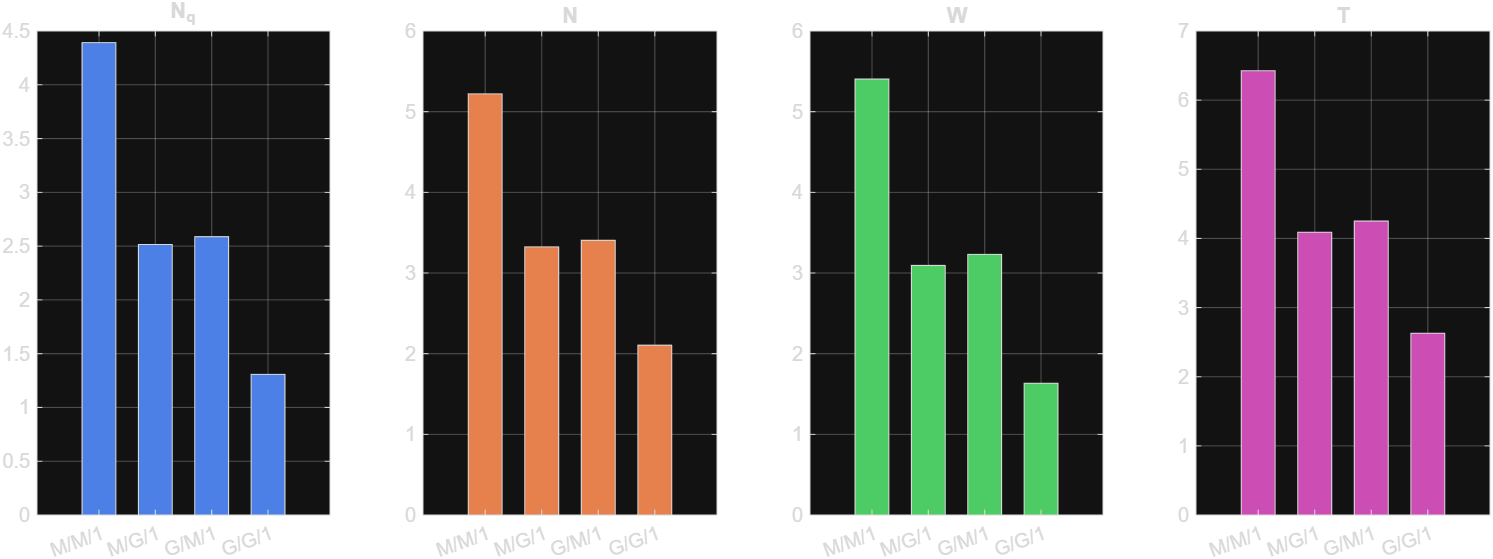
\includegraphics[width=0.98\textwidth]{lab7_fig1.png}
    \caption{Система M/M/1: приход/обслуживание, число заявок во времени, распределение числа заявок}
    \label{fig:lab7_mm}
\end{figure}

\begin{figure}[H]
    \centering
    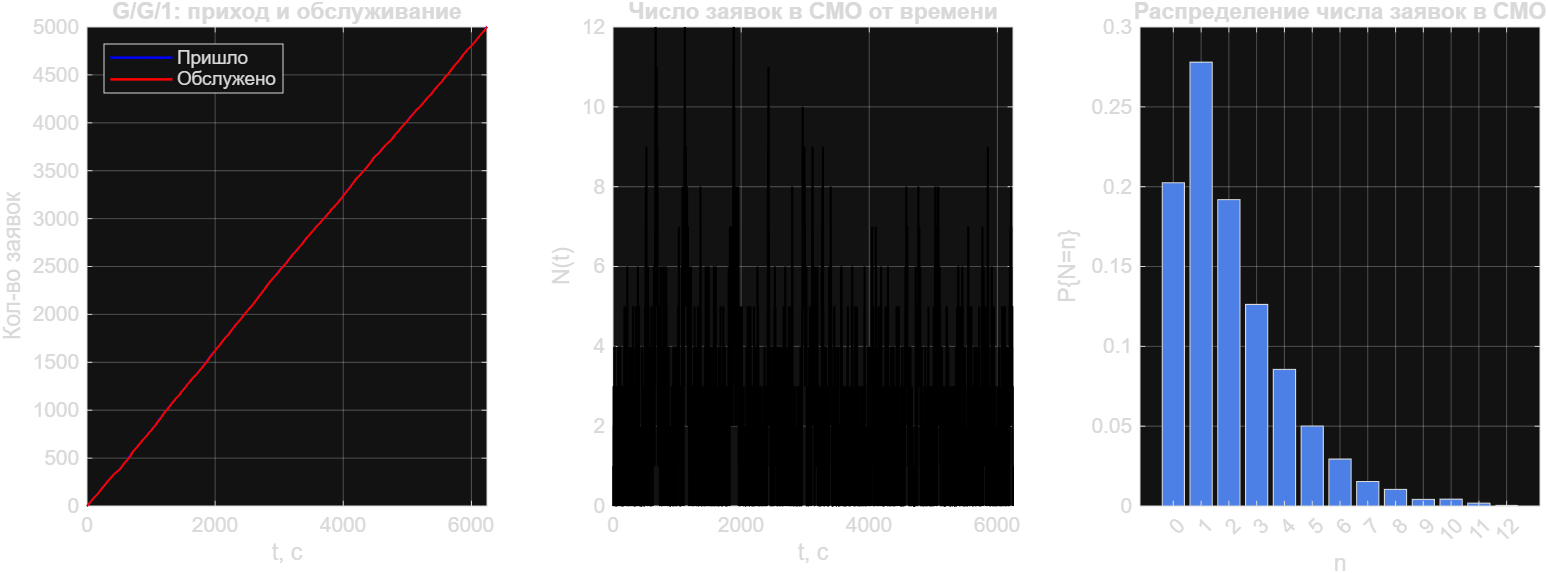
\includegraphics[width=0.98\textwidth]{lab7_fig2.png}
    \caption{Система M/G/1}
    \label{fig:lab7_mg}
\end{figure}

\begin{figure}[H]
    \centering
    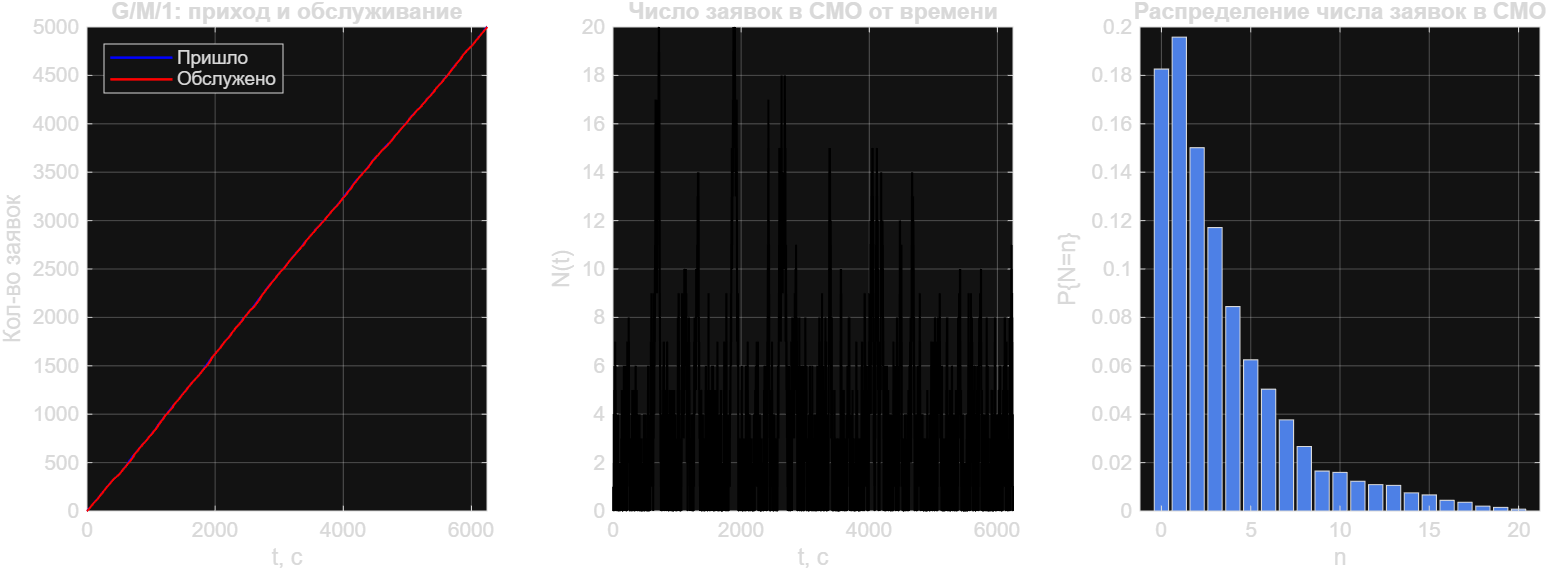
\includegraphics[width=0.98\textwidth]{lab7_fig3.png}
    \caption{Система G/M/1}
    \label{fig:lab7_gm}
\end{figure}

\begin{figure}[H]
    \centering
    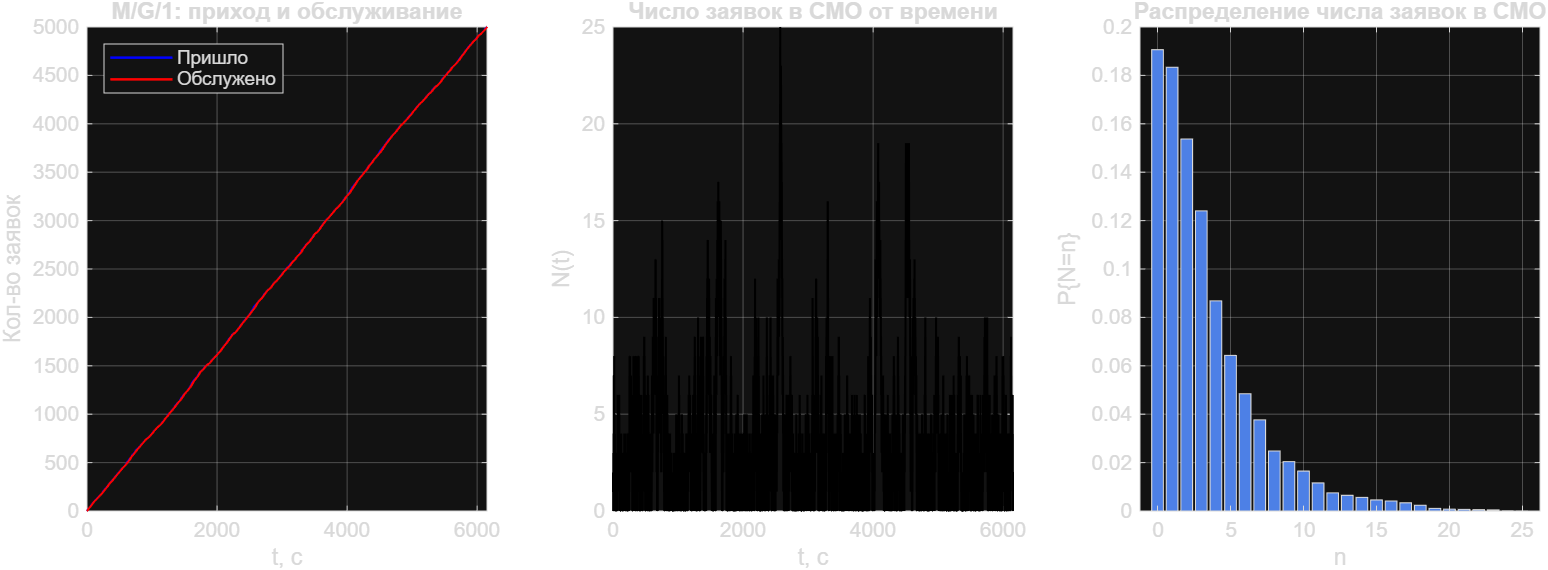
\includegraphics[width=0.98\textwidth]{lab7_fig4.png}
    \caption{Система G/G/1}
    \label{fig:lab7_gg}
\end{figure}

Сводное сравнение характеристик четырёх типов представлено на рис.~\ref{fig:lab7_cmp}.

\begin{figure}[H]
    \centering
    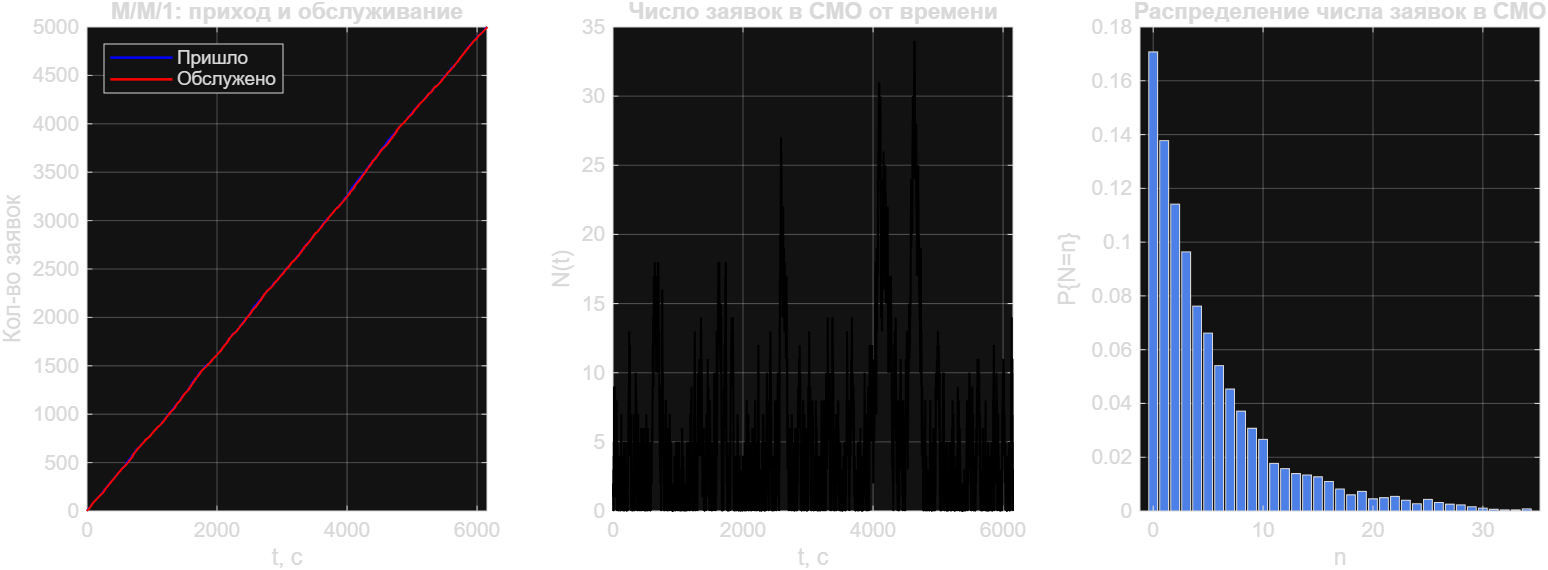
\includegraphics[width=0.98\textwidth]{lab7_fig5.png}
    \caption{Сравнение характеристик $N_q$, $N$, $W$, $T$ для четырёх типов СМО}
    \label{fig:lab7_cmp}
\end{figure}

\textbf{Анализ.} Наибольшие значения $N_q$, $N$, $W$, $T$ даёт система M/M/1 --- обе последовательности имеют максимальную дисперсию. Замена обслуживания на менее вариативное гамма-распределение (M/G/1) снижает среднее число заявок примерно в 1,6 раза. Регулярный вход (G/M/1) также уменьшает очередь. Минимальные характеристики --- у G/G/1, где и вход, и обслуживание менее случайны. Таким образом, чем меньше дисперсия управляющих последовательностей, тем короче очередь и меньше время пребывания, что и подтверждает имитация.

\section*{Ответы на контрольные вопросы}
\begin{enumerate}
    \item \textbf{Классификация СМО.} По числу каналов (одноканальные/многоканальные), по очереди (с ограниченной/неограниченной очередью, с отказами, с ожиданиями), по дисциплине обслуживания (FIFO, LIFO, приоритеты), по законам распределения входного потока и обслуживания.
    \item \textbf{Обозначения СМО.} Нотация Кендалла $A/B/n/m$: $A$ --- закон входного потока, $B$ --- закон обслуживания, $n$ --- число каналов, $m$ --- ёмкость; $M$ --- показательный, $D$ --- детерминированный, $G$ --- произвольный.
    \item \textbf{Входной поток и процесс обслуживания.} Входной поток --- последовательность интервалов $\{\tau_n\}$ между заявками; процесс обслуживания --- последовательность $\{\nu_n\}$ длительностей обслуживания.
    \item \textbf{Условие стационарности.} Среднее число поступлений должно быть меньше производительности: $\rho=\lambda/\mu<1$. Иначе очередь неограниченно растёт.
    \item \textbf{Коэффициент загрузки.} $\rho=\lambda/\mu$ --- доля времени занятости канала, совпадает со средним числом занятых каналов.
    \item \textbf{Распределение числа требований в системе.} Стационарные вероятности $P_n$ нахождения $n$ заявок в системе; для M/M/1 --- геометрическое $P_n=(1-\rho)\rho^n$.
    \item \textbf{Состояния СМО.} Число заявок в системе $n=0,1,2,\dots$; переходы между состояниями происходят в моменты поступления и окончания обслуживания.
    \item \textbf{Зависимость характеристик от распределений.} Характеристики зависят не только от средних $\lambda,\mu$, но и от дисперсий: бо\'льшая вариативность входа/обслуживания увеличивает очередь и время пребывания (формула Хинчина--Поллячека).
\end{enumerate}

\section{Текст программы}
\begin{verbatim}
%% Лабораторная работа N7. ИКС-431 Салий В.П., вариант 18
lambda = 0.8;  mu = 1.0;  N = 5000;

% Управляющие последовательности (как в лаб. 6)
tau  = -log(rand(N,1)) / lambda;     % показательный вход
nu   = -log(rand(N,1)) / mu;         % показательное обслуживание
E_tau = 1/lambda;  D_tau = 1/lambda^2;
E_nu  = 1/mu;      D_nu  = 1/mu^2;
b_tau = (D_tau/2)/E_tau;  c_tau = E_tau^2/(D_tau/2);
b_nu  = (D_nu /2)/E_nu ;  c_nu  = E_nu ^2/(D_nu /2);
tau1 = my_gamrnd(c_tau, b_tau, N);   % гамма-вход
nu1  = my_gamrnd(c_nu,  b_nu,  N);   % гамма-обслуживание

types = {'M/M/1','M/G/1','G/M/1','G/G/1'};
ins = {tau, tau, tau1, tau1};
svs = {nu,  nu1, nu,   nu1};
for t = 1:4
    r = sim_smo(ins{t}, svs{t});
    fprintf('%s: rho=%.3f N=%.3f W=%.3f T=%.3f\n', ...
        types{t}, r.rho, r.N, r.W, r.T);
end

function out = sim_smo(tau, nu)
    N = numel(tau);  arr = cumsum(tau);
    dep = zeros(N,1);  wait = zeros(N,1);  free = 0;
    for i = 1:N
        a = arr(i);
        if free <= a, w_i = 0; free = a + nu(i);
        else, w_i = free - a; free = free + nu(i); end
        wait(i) = w_i;  dep(i) = free;
    end
    out.T = mean(dep - arr);  out.W = mean(wait);
    lam = N / dep(end);
    out.N = lam*out.T;  out.Nq = lam*out.W;  out.rho = lam*mean(nu);
    % ступенчатая функция числа заявок и её распределение ...
end
\end{verbatim}

\section*{Выводы по лабораторной работе}
\addcontentsline{toc}{section}{Выводы по лабораторной работе}
Методом дискретно-событийного моделирования исследованы четыре одноканальные СМО (M/M/1, M/G/1, G/M/1, G/G/1), построенные на управляющих последовательностях из лабораторной работы №6. Для каждой модели получены зависимости числа пришедших и обслуженных заявок от времени, числа заявок в СМО от времени и распределение числа заявок, а также статистические характеристики $\rho$, $N_q$, $N$, $W$, $T$.

Показано, что вероятностно-временные характеристики СМО существенно зависят от типа (дисперсии) законов распределения входного потока и обслуживания: максимальную очередь даёт система M/M/1, минимальную --- G/G/1. Уменьшение вариативности входного потока или времени обслуживания снижает среднее число заявок и время пребывания, что согласуется с формулой Хинчина--Поллячека. Для всех систем выполняется формула Литтла $N=\lambda T$, а условие стационарности $\rho<1$ соблюдается.

\end{document}
